\documentclass[a4paper,11pt]{article}
\usepackage[utf8]{inputenc}
\usepackage{graphicx}
\usepackage{hyperref}
\usepackage[fontset=windows]{ctex} % Set `fontset` to your system fontset (windows, mac, ubuntu etc.)
\usepackage{amsmath}
\usepackage{amssymb}
\usepackage{listings}
\usepackage{xcolor}
\usepackage{graphicx}
\usepackage{amsmath}
\usepackage{amsfonts}
\usepackage{xcolor}  % 颜色控制包
\title{说明文档:AnaClock-React}
\date{}

\begin{document}

\maketitle

\tableofcontents
\newpage
\section{实现思路}
\subsection{时钟}
\subsubsection{时钟组件}\label{subsec:clock}
采用单向数据流实现时钟组件。

时钟三个指针的角度由当前的时间戳唯一决定。基于这一点,我们让时钟组件接受一个时间戳作为参数,在组件内部根据时间戳绘制不同角度的指针。时间戳的具体值由父组件(如时钟标签页、闹钟标签页等)决定。
\subsubsection{平滑效果}
采用高频更新的方式实现平滑效果。

时钟组件实际上是静态的。时钟组件内部并不会自动移动指针。指针在视觉上的走动效果实际上来源于父组件定时更新时钟组件的时间戳参数。为了达到指针平滑走动的效果,我们选择父组件每隔 16 ms 更新一次时间戳,这样可以做到每秒 60 帧的指针走动,从而达到平滑效果。

\subsubsection{拖拽功能}
使用 d3.js 组件库实现拖拽功能,

使用回调函数更新父组件时间戳。d3.js 是一个常用于绘图的 JS 组件库。定义一个 d3 的 DragBehavior, 在拖动过程中,behavior 会调用自定义的函数,根据当前鼠标的位置和上一个时刻指针的位置,计算指针新的位置。在拖动结束时,behavior 会调用一个回调函数,用于将当前的指针所指的时间戳赋值给父组件中的时间戳。另外,我们对拖动指针跨越 0 点时的角度做了特殊处理。可以正确地在拖动中切换上下午。


\subsection{闹钟}
\subsubsection{时钟组件}
与\ref{subsec:clock}中基本相同,但为了保证时间的精确以及闹钟的有效提醒,在alarmTab页面禁用了闹钟的拖拽功能。
\subsubsection{添加功能}
使用AddButton组件用于添加新的闹钟,其本质是一个包含FAB按钮及其相关处理逻辑的组件(代码位于app/components/addButton.tsx中)。在AddButton中,我们使用了MUI风格的Fab组件来实现悬浮按钮,并通过Zoom组件实现了逐渐显示的动画效果。点击FAB按钮后,将弹出用于添加闹钟的对话框。对话框基于MUI的Dialog组件实现。打开对话框后,如果添加成功或取消操作,均会给出不同的提示,这些提示框采用了MUI的SnackBar和Alert组件。在成功添加闹钟后,将闹钟信息保存到LocalStorage中。
\subsubsection{闹钟功能}
使用Alarms组件用于在alarmTab页面的右侧显示当前闹钟列表并处理相关逻辑(代码见app/components/alarms.tsx),每个闹钟条目由AlarmItem组件表示(代码位于app/components/alarmItem.tsx,样式位于app/components/alarmItem.module.css)。在Alarms中,我们实现了点击某个闹钟可以对该闹钟进行编辑,包括重新命名和更改时间。编辑方式类似于添加闹钟的对话框。此外,我们也实现了通过AlarmItem右侧的switchButton来决定是否启用闹钟,只有当switchButton切换为打开(绿色)时,闹钟才会响铃。为了提示闹钟时间到达,我们每秒检查一次当前系统时间是否与LocalStorage中的某个闹钟时间相同。提示方式采用了与计时器时间到达提示一致的方式,包括一个位于屏幕中心的MUI-Dialog提示,以及右下角的系统提示。
\subsection{计时器}
\subsubsection{时钟组件}
与\ref{subsec:clock}中基本相同,但为了切合计时器的功能,改变了时间的获取。
\subsubsection{计时功能}
使用 React 的 useState 钩子初始化包括 timeStamp(当前时间戳)、pause(是否暂停)和 editing(是否处于编辑状态)在内的状态。通过 useEffect 设置一个定时器,每隔 16 毫秒更新一次时间戳,模拟时间流逝。若时间戳降至 0 或以下,则发送通知,用户可交互地通过界面上的按钮控制计时器的开始、暂停和时间编辑。
\subsubsection{通知功能}
\textbf{界面通知:}
使用 Dialog 组件提供计时结束时的界面反馈,并且同样通过 useEffect 设
置一个定时器,每隔 16 毫秒更新一次时间戳,模拟时间流逝,以此来实时更新超时时长。

\textbf{系统通知:}
若用户已授权,使用Notification 组件发送桌面通知,并设置点击回到原始界面,而非新开一个界面。
\subsection{秒表}
\subsubsection{时钟组件}
与\ref{subsec:clock}中基本相同,但同样为了切合秒表的功能,改变了时间的获取。
\subsubsection{计时功能}
计时功能依赖于 React 的 useState 钩子来初始化当前时间戳(timeStamp)和暂停状态(pause)。通过 useEffect 设置一个定时器,每 16 毫秒更新一次时间戳,模拟计时器的运行。计时期间,时间格式化函数 formatTime 将时间戳转换为易读的格式(日、时、分、秒、毫秒)。主题变化通过 useTheme 钩子动态调整,以适应不同的用户偏好。
\subsubsection{标记功能}
标记功能允许用户在计时过程中通过点击“标记”按钮记录当前时间点,通过 handleLap 函数将当前时间添加到标记列表(laps)。标记列表以表格形式展示,每个标记显示序号和时间。表格使用 TableContainer 组件实现,支持滚动,并随着新标记的添加自动滚动到顶部。按钮逻辑通过条件渲染实现,根据计时状态切换显示“复位/启动”或“标记/暂停”。
\subsection{明暗模式切换}
使用 \texttt{next-themes} 包通过命令 \texttt{npm install next-themes} 进行安装。在 \texttt{app/layout.tsx} 中引入 \texttt{ThemeProvider} 并设置 \texttt{attribute="class"} 属性,允许主题直接影响 CSS 类。在 \texttt{app/globals.css} 中定义 CSS 变量和属性,通过类 \texttt{.dark} 和 \texttt{.light} 设置如背景色和文本色的变量:
\begin{verbatim}
.dark {
  --backgroundColor: black;
  --textColor: white;
  background-color: black;
}
\end{verbatim}

在其他页面或组件中,使用在 \texttt{globals.css} 中声明的 CSS 变量来处理组件在不同主题模式下的颜色,例如使用 \texttt{var(--textColor)}。对于 Material-UI 组件,使用 \texttt{MUIThemeProvider} 来应用主题,在 \texttt{app/muiThemes.tsx} 中定义了 \texttt{lightTheme} 和 \texttt{darkTheme},并在页面或组件中通过 \texttt{useTheme} (导入自 \texttt{next-themes})获取当前系统主题,根据该主题决定使用 \texttt{lightTheme} 或 \texttt{darkTheme}。
\section{使用说明}
\subsection{简介}
本应用包含时钟、闹钟、计时器、秒表以及明暗模式切换功能。

\subsection{时钟}
\subsubsection{表盘}
如图\ref{fig:clock}所示,在时钟界面中含有指针式表盘以及数字式表盘,两个表盘的时间总是保持一致

其中在指针式表盘中含有时针、分针和秒针(秒针按照要求设计为红色),支持秒针在刻度之间平滑移动。
\begin{figure}[!h]
    \centering
    \begin{minipage}{0.7\textwidth}
        \centering
        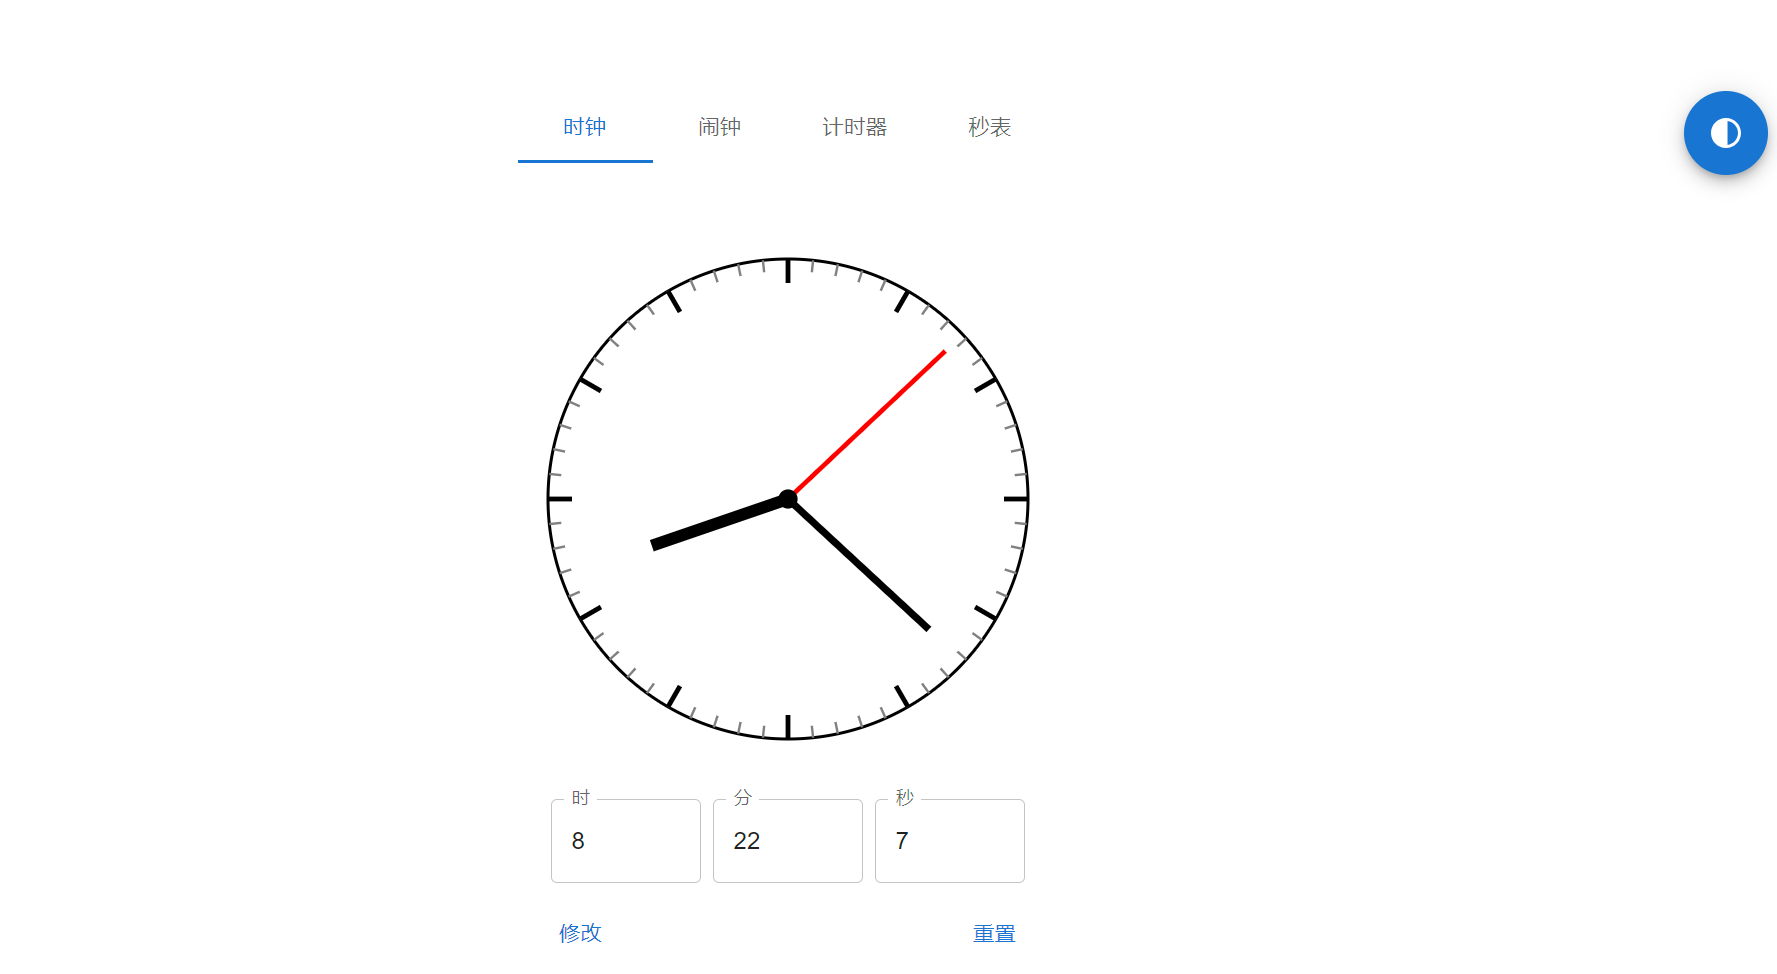
\includegraphics[width=\linewidth]{image/clock.png}
        \caption{clock}
            \label{fig:clock}
    \end{minipage}
\end{figure}
\subsubsection{更改时间}
在图\ref{fig:clock}中可支持通过指针式表盘或是数字式表盘更改时间:
\begin{itemize}
  \item 指针式表盘:可直接通过鼠标拨动时针、分针和秒针来更改时间;
  \item 数字式表盘:可通过点击“修改”,再直接在数字式表盘中更改时间。
  \item 点击“重置”后可使两个表盘时间回到显示北京时间。
\end{itemize}

\subsection{闹钟}

\subsubsection{添加闹钟}
在图\ref{fig:alarm}中,点击“+”按钮后进入图\ref{fig:alarm_add},进行添加闹钟操作,在确定好时间后,点击“确认”即可在右方看到设置的闹钟。
\begin{figure}[!h]
    \centering
    \begin{minipage}{0.48\textwidth}
        \centering
        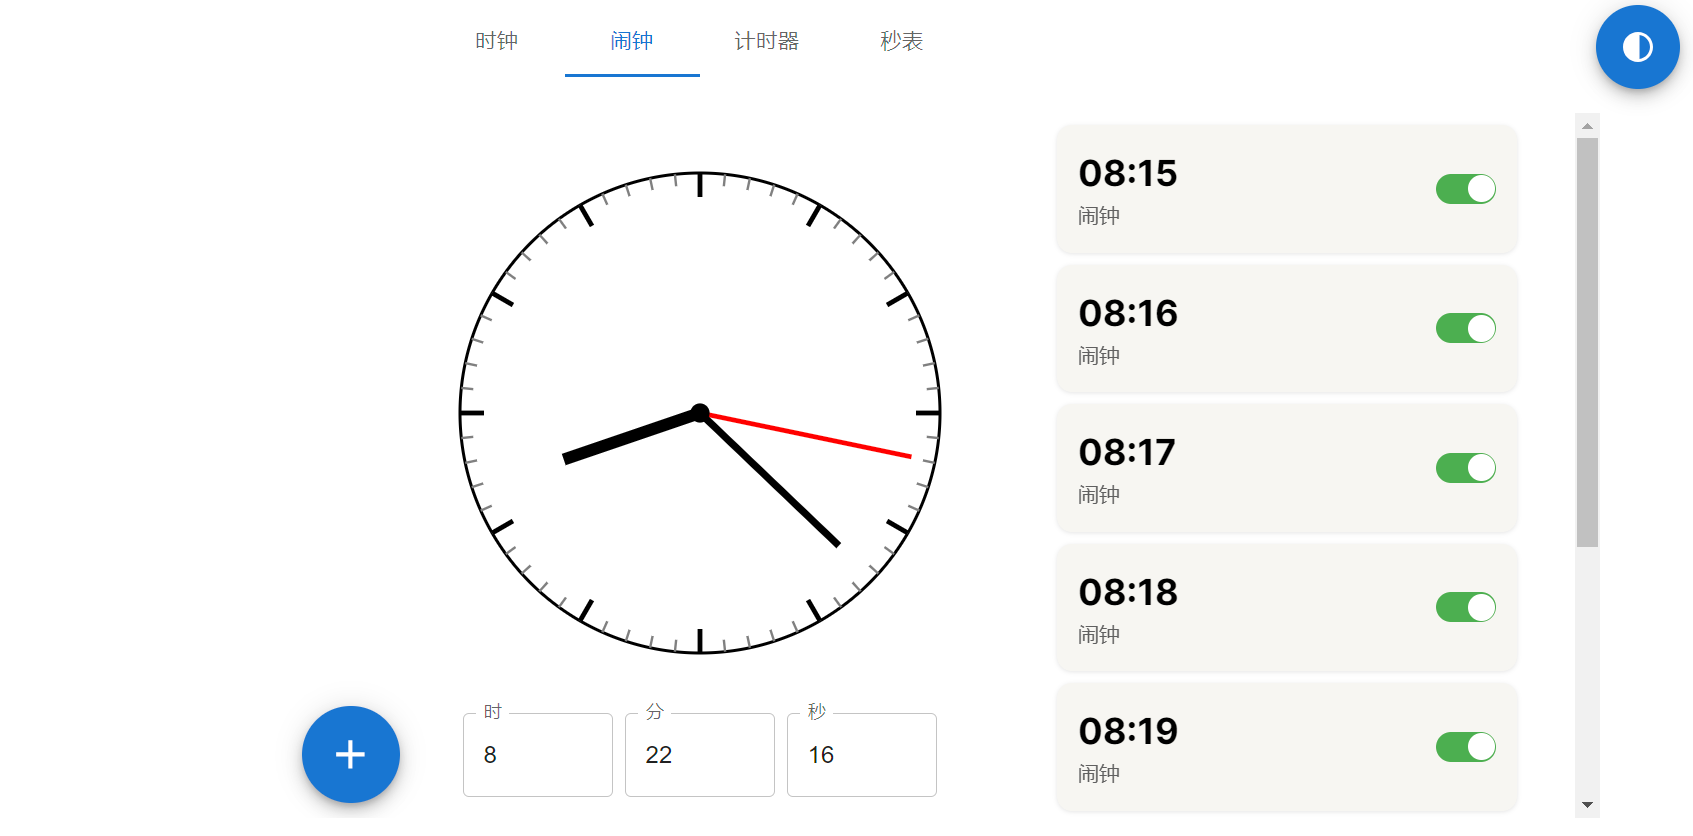
\includegraphics[width=\linewidth]{image/alarm.png}
        \caption{alarm}
            \label{fig:alarm}
    \end{minipage}\hfill
    \begin{minipage}{0.48\textwidth}
        \centering
        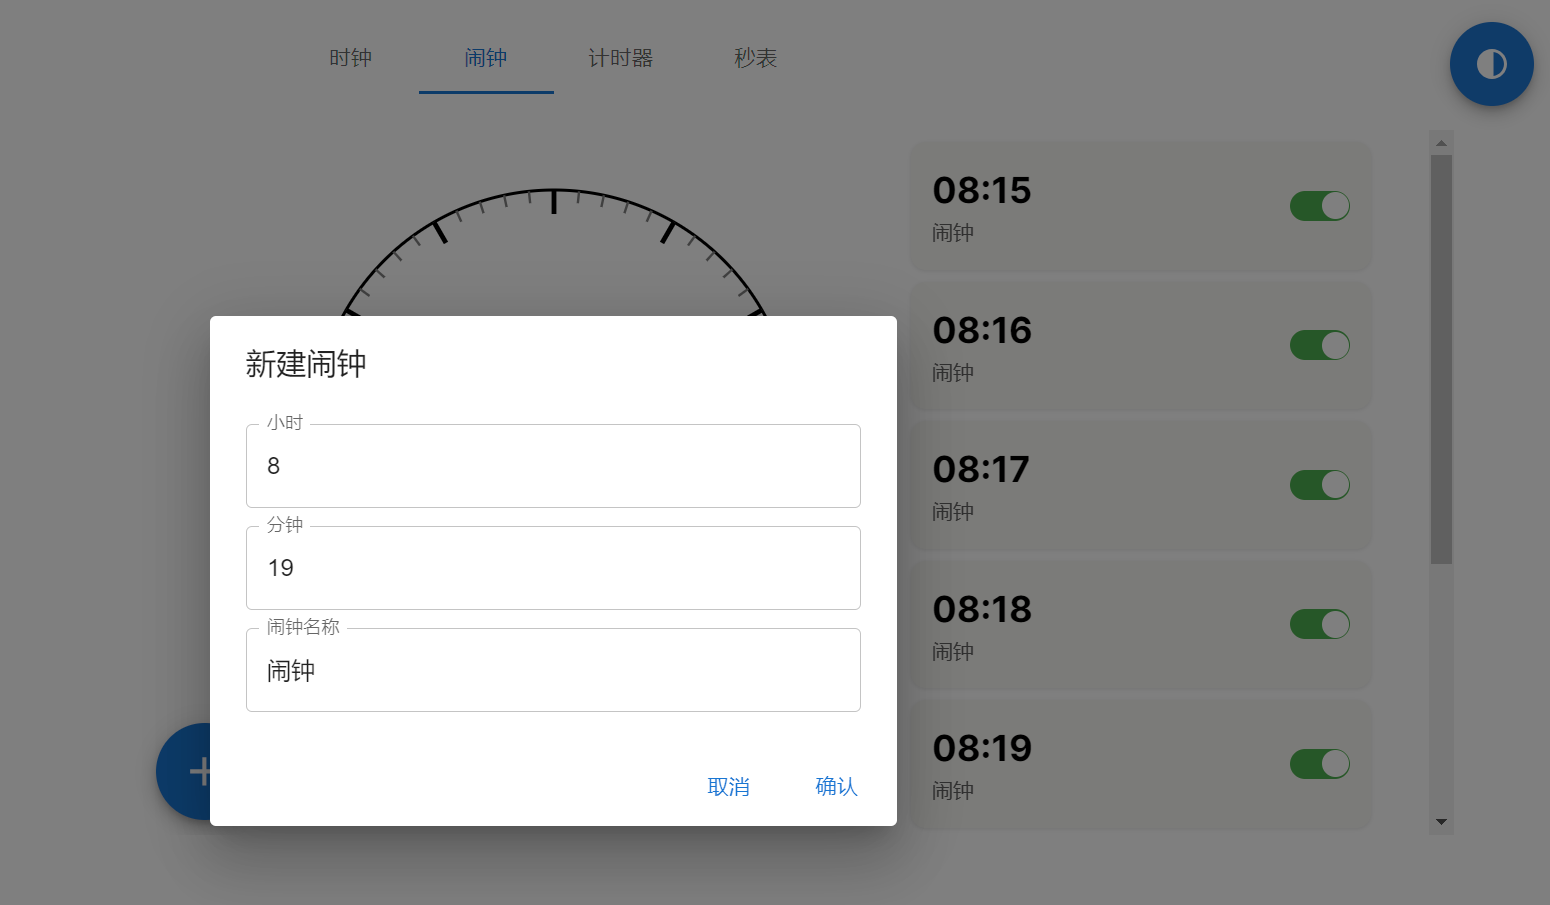
\includegraphics[width=\linewidth]{image/alarm_add.png}
        \caption{alarm\_add}
        \label{fig:alarm_add}
    \end{minipage}
\end{figure}

\subsubsection{编辑闹钟}
在图\ref{fig:alarm}中,点击右方闹钟处的滑动开关可控制闹钟的开启与关闭

直接点击闹钟可进入图\ref{fig:alarm_edit}进行闹钟编辑,包含“更改时间”以及“删除闹钟”功能
\subsubsection{闹钟响起}\label{subsec:alarm}
当到达某一闹钟设置的时间后,将会显示图\ref{fig:alarm_tri},弹出两个通知,分别为界面通知和系统通知,

\begin{itemize}
  \item 界面通知:即图\ref{fig:alarm_tri}正中间的通知,可显示距离闹钟响起过去了多长时间,点击界面的任意处即可关闭。
  \item 系统通知:即图\ref{fig:alarm_tri}右下角的通知,点击后可以回到闹钟界面。
\end{itemize}

\begin{figure}[!h]
    \centering
    \begin{minipage}{0.48\textwidth}
        \centering
        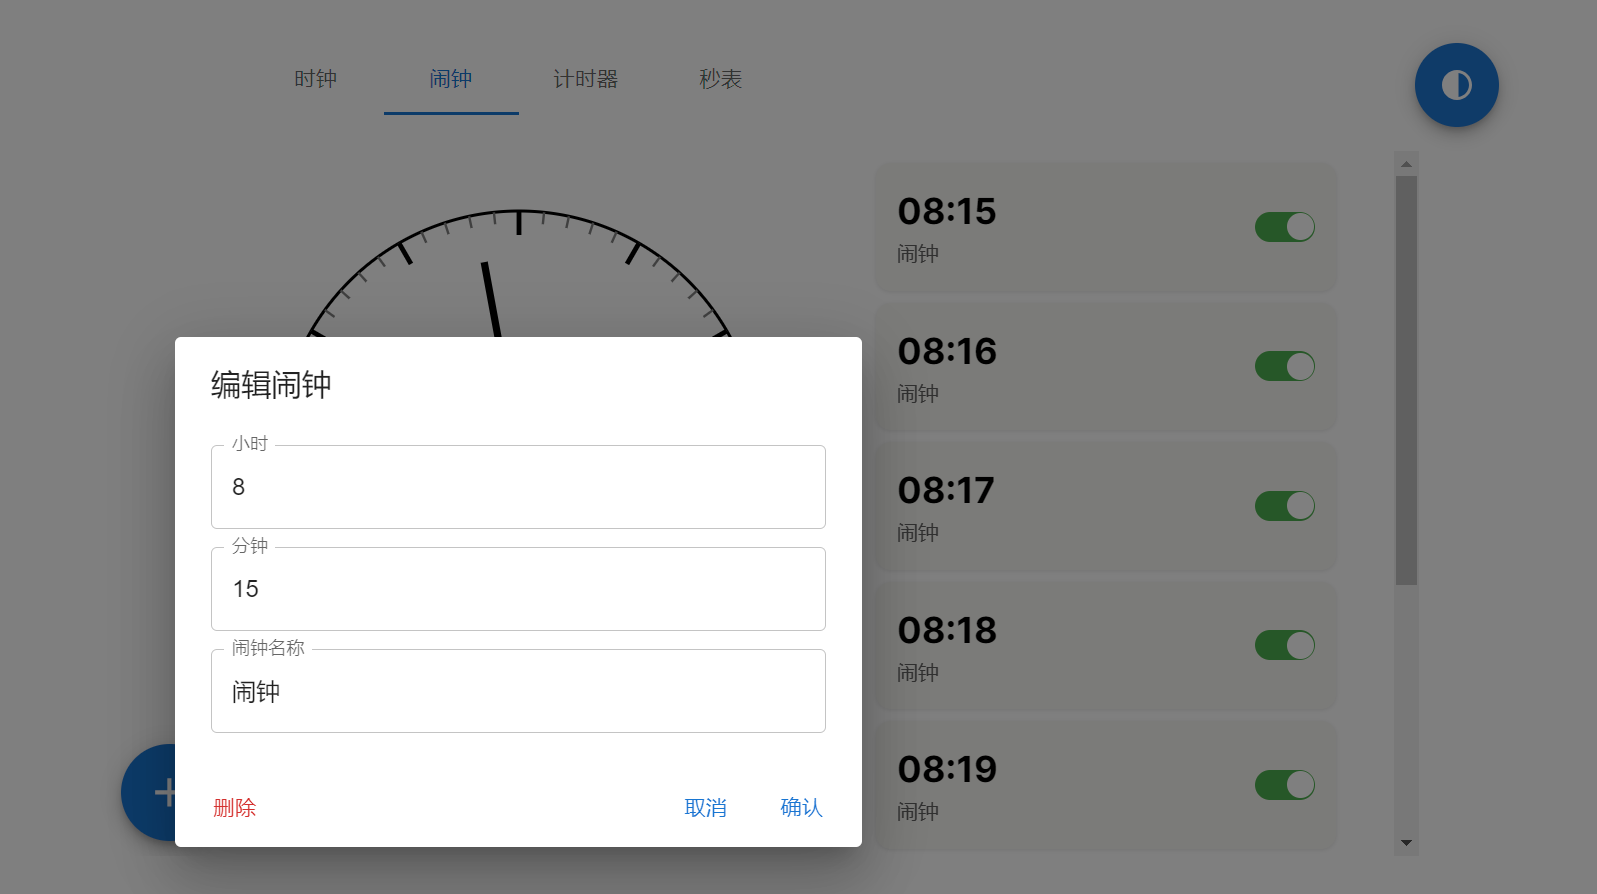
\includegraphics[width=\linewidth]{image/alarm_edit.png}
        \caption{alarm\_edit}
            \label{fig:alarm_edit}
    \end{minipage}\hfill
    \begin{minipage}{0.48\textwidth}
        \centering
        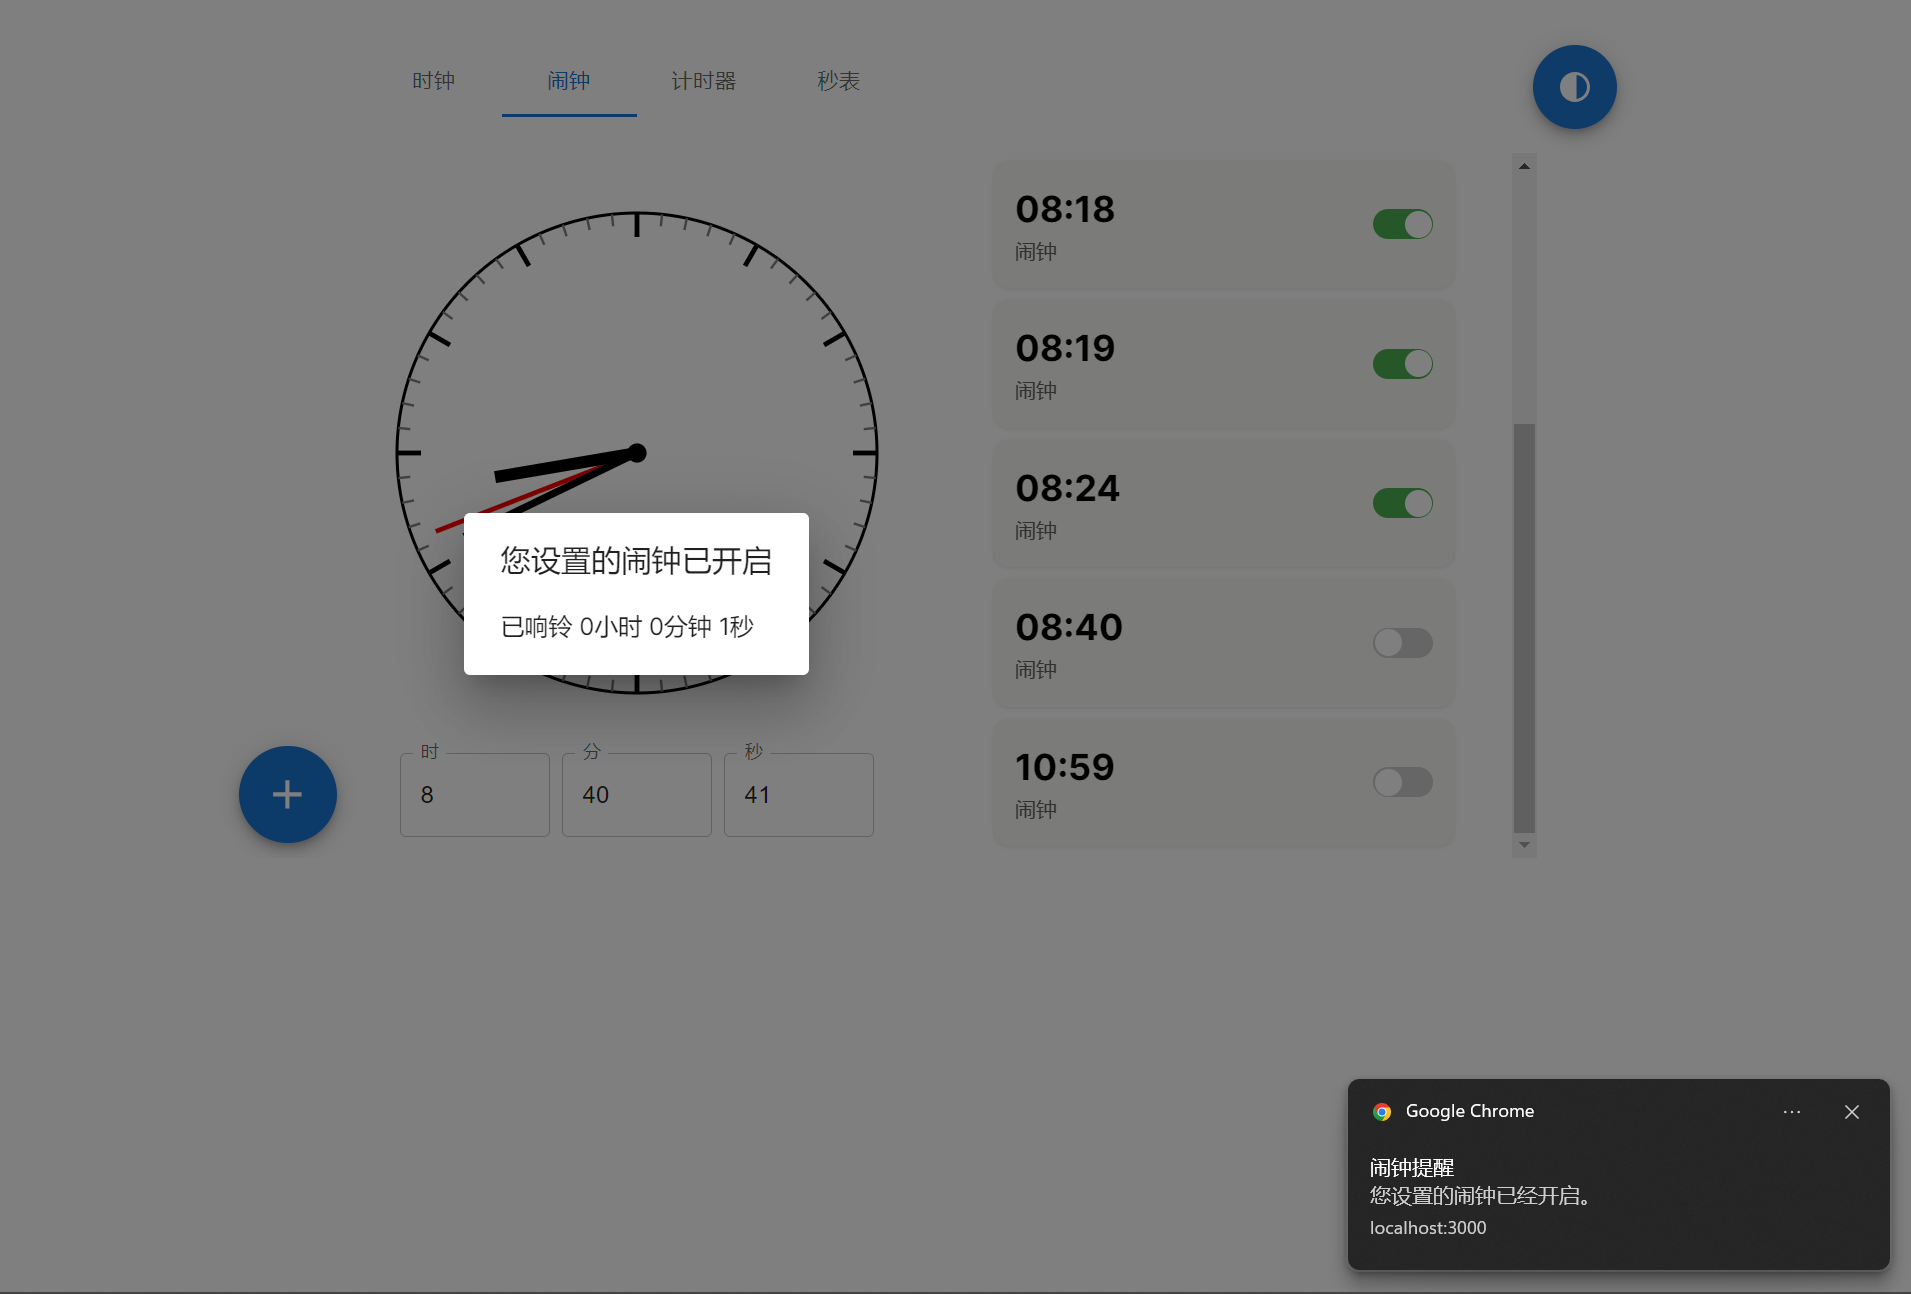
\includegraphics[width=\linewidth]{image/alarm_trigger.png}
        \caption{alarm\_tri}
        \label{fig:alarm_tri}
    \end{minipage}
\end{figure}


\subsection{计时器}
\subsubsection{计时功能}
在图\ref{fig:timer}中,点击“编辑”按钮即可编辑计时器的时间,“恢复”和“暂停”按钮可控制计时器的开启与关闭。
\subsubsection{计时器响起}
计时器时间归零后,进入图\ref{fig:timer_tri},弹出两个通知,分别为界面通知和系统通知,与 \ref{subsec:alarm}中功能相同。

\begin{figure}[!h]
    \centering
    \begin{minipage}{0.48\textwidth}
        \centering
        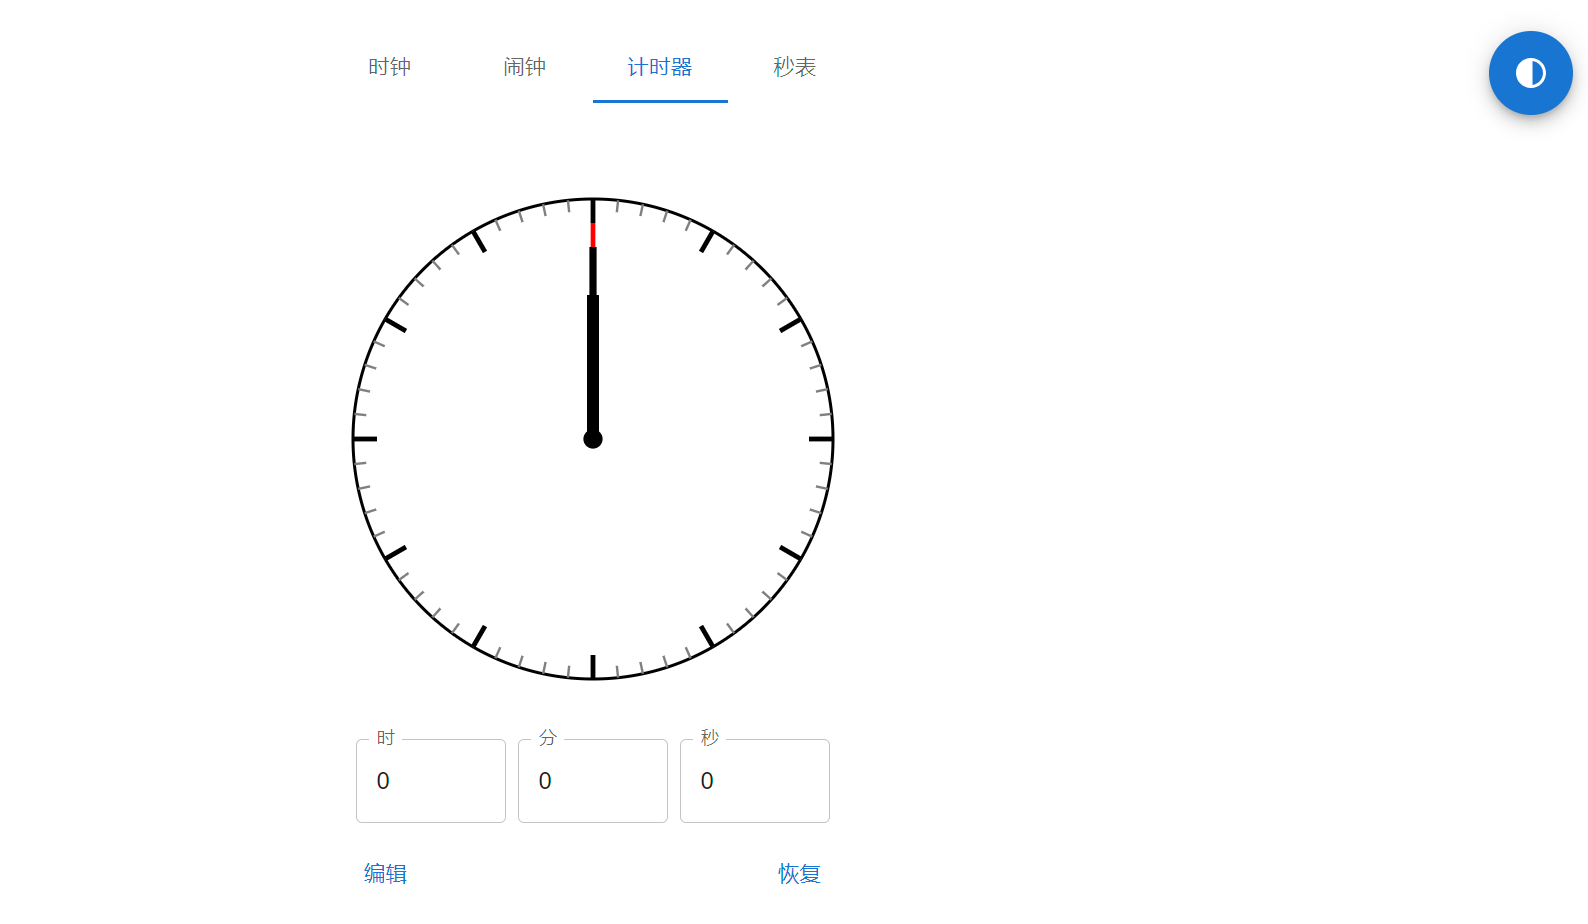
\includegraphics[width=\linewidth]{image/timer.png}
        \caption{timer}
            \label{fig:timer}
    \end{minipage}\hfill
    \begin{minipage}{0.48\textwidth}
        \centering
        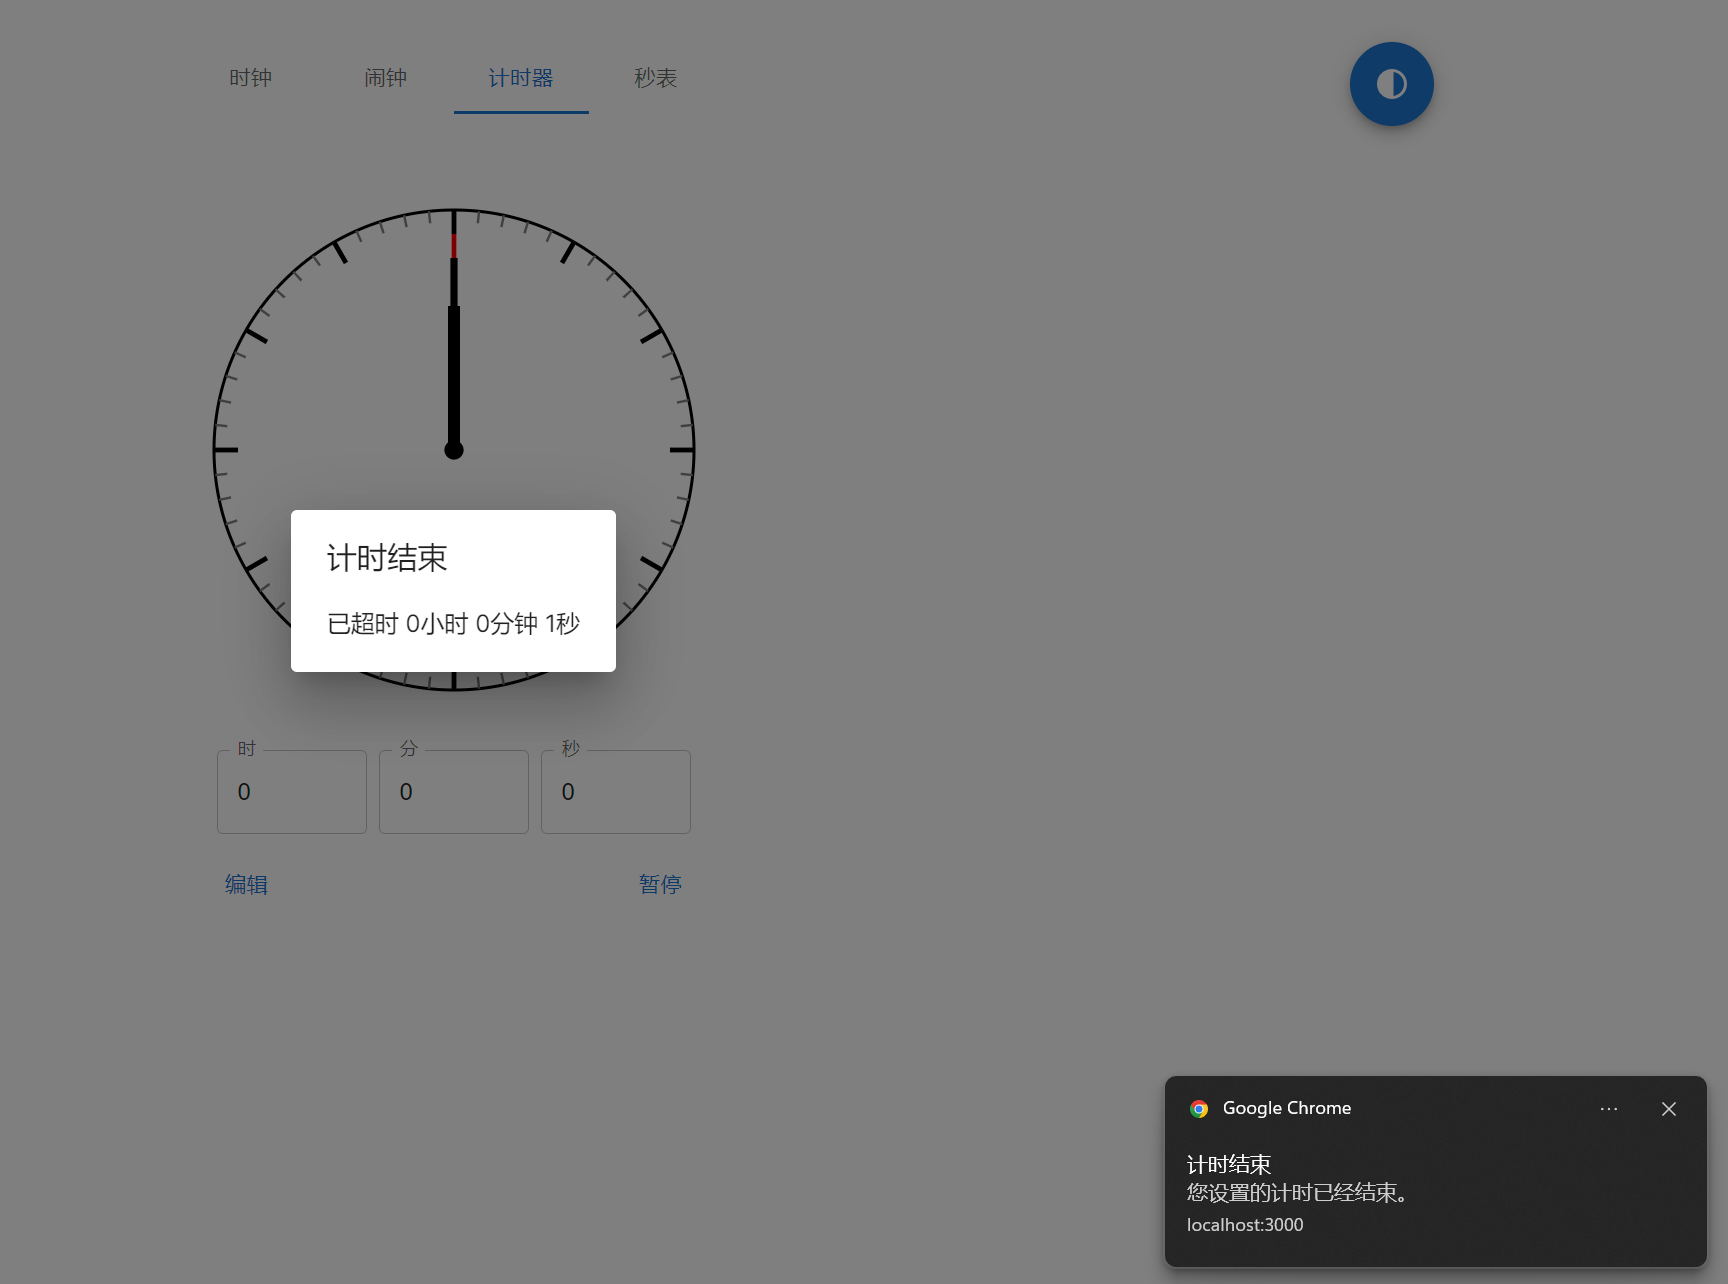
\includegraphics[width=\linewidth]{image/timer_tri.png}
        \caption{timer\_tri}
        \label{fig:timer_tri}
    \end{minipage}
\end{figure}

\subsection{秒表}
\subsubsection{计时功能}
在图\ref{fig:stopwatch}中,点击“启动”按钮即可开始计时,开始计时后可通过“暂停”和“复位”按钮来停止计时和重置计时。
\subsubsection{标记功能}
在开始计时后,可点击“标记”按钮来记录时间,效果如图\ref{fig:stopwatch_time},在点击“复位”后记录消失。

\begin{figure}[!h]
    \centering
    \begin{minipage}{0.48\textwidth}
        \centering
        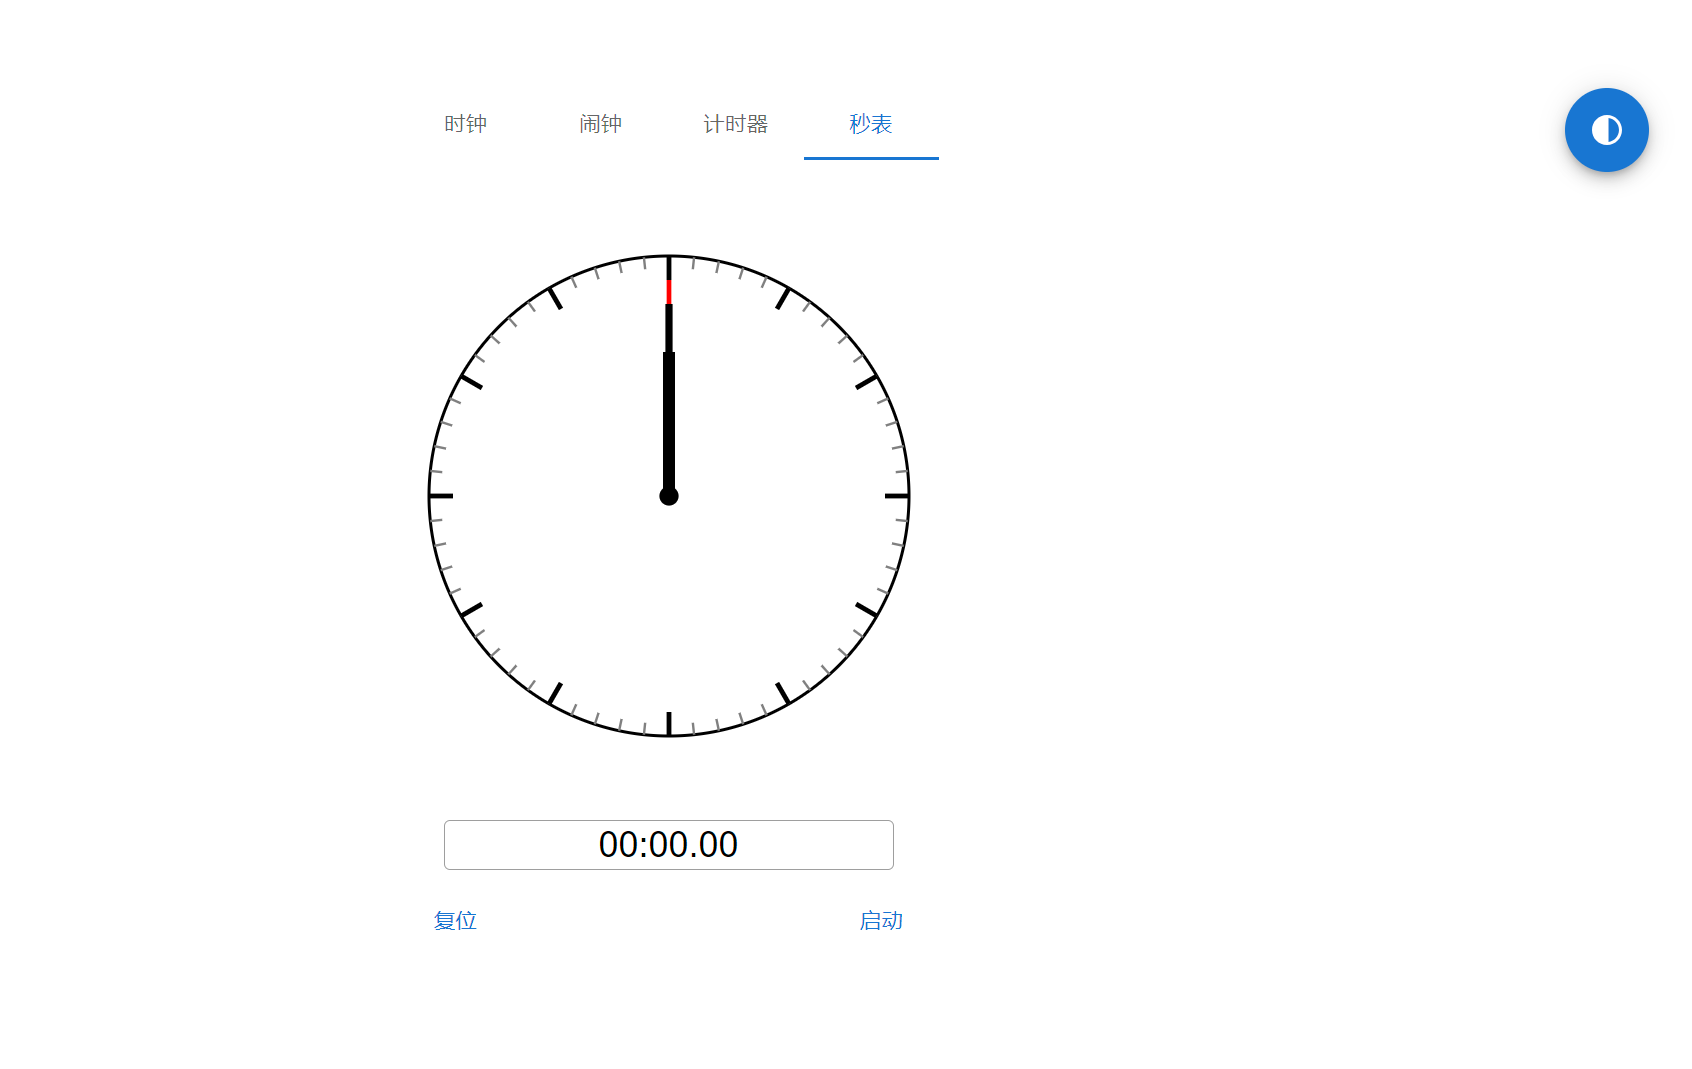
\includegraphics[width=\linewidth]{image/stopwatch.png}
        \caption{stopwatch}
            \label{fig:stopwatch}
    \end{minipage}\hfill
    \begin{minipage}{0.48\textwidth}
        \centering
        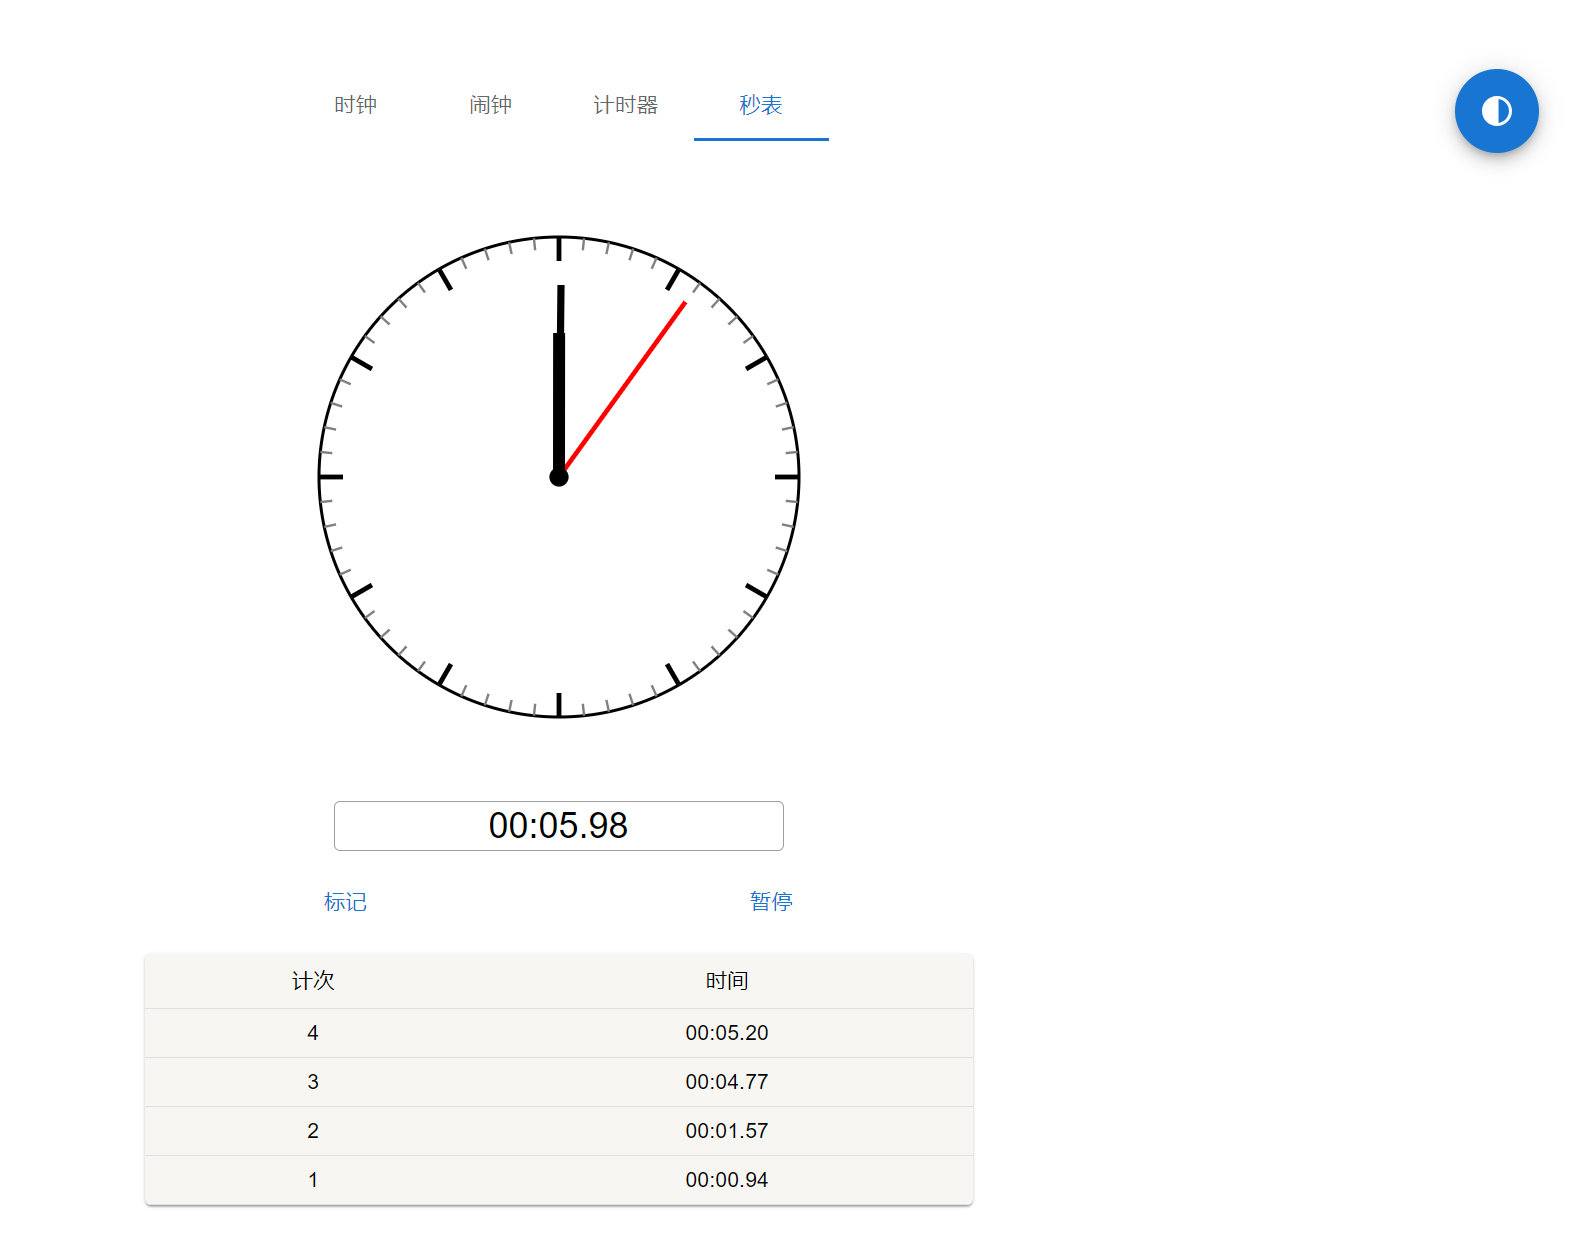
\includegraphics[width=\linewidth]{image/stopwatch_time.png}
        \caption{stopwatch\_time}
        \label{fig:stopwatch_time}
    \end{minipage}
\end{figure}

\subsection{明暗模式切换}
在每个界面的右上角存在“明暗模式切换按钮”,点击可更改为明亮或是黑暗模式,下面为效果对比图

\begin{figure}[!h]
    \centering
    \begin{minipage}{0.48\textwidth}
        \centering
        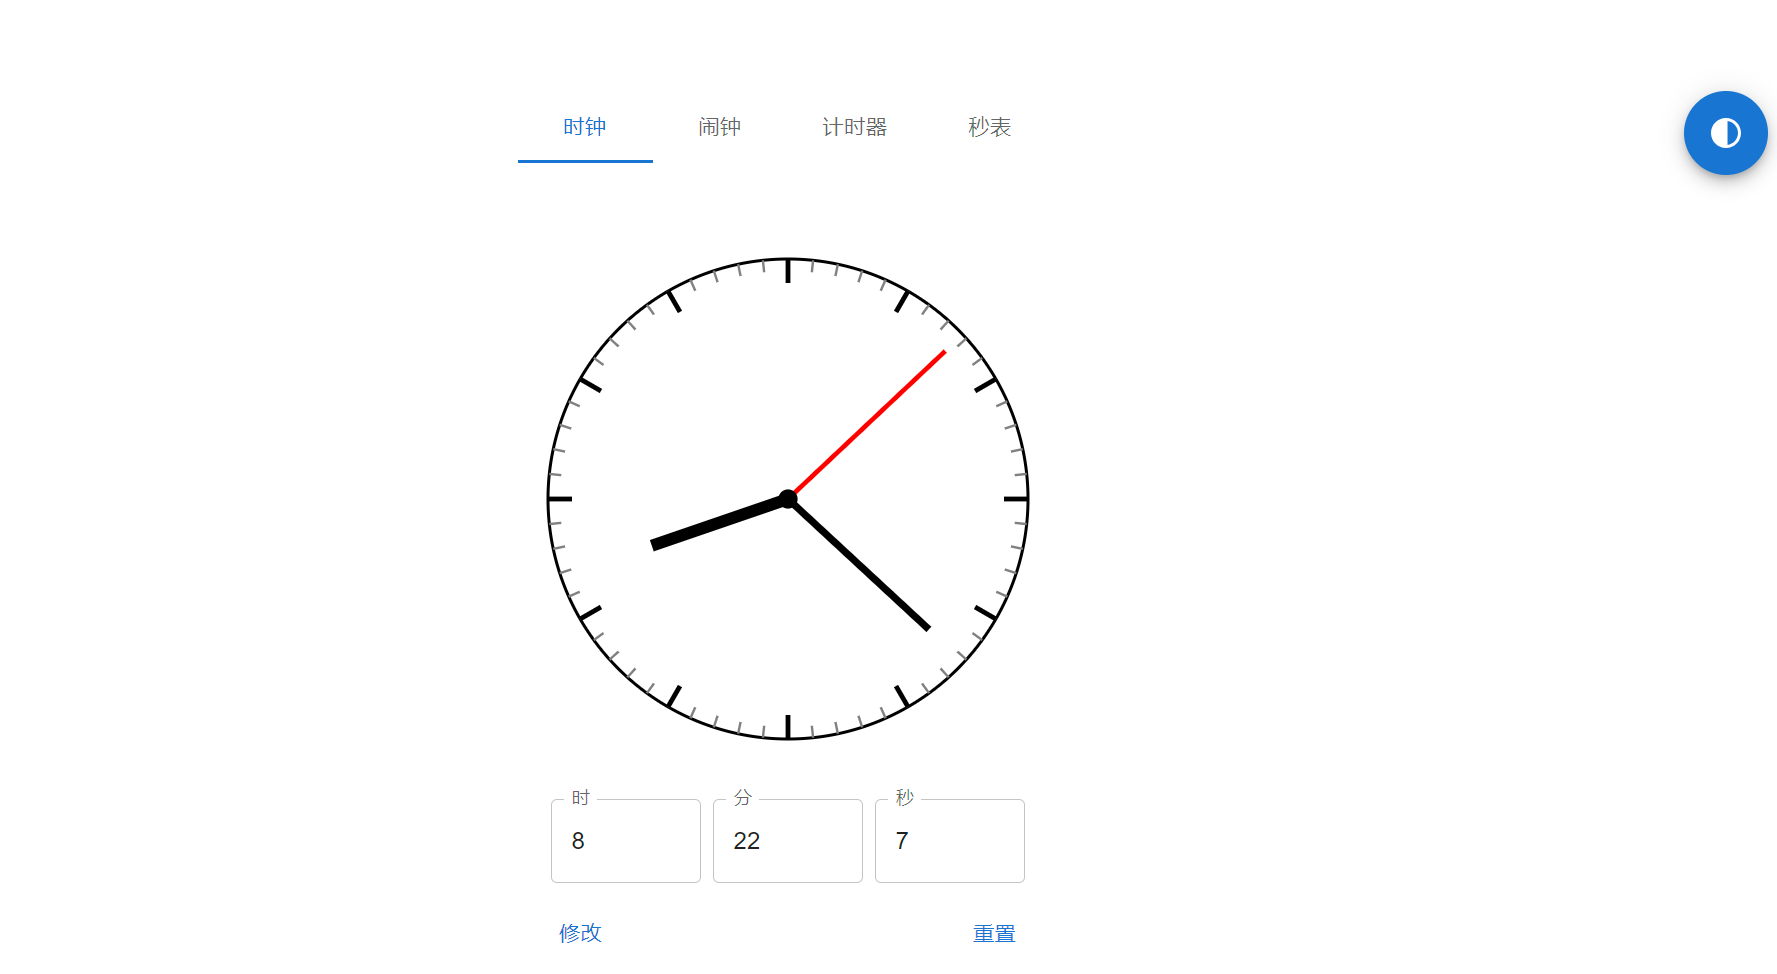
\includegraphics[width=\linewidth]{image/clock.png}
        \caption{clock\_light}
    \end{minipage}\hfill
    \begin{minipage}{0.48\textwidth}
        \centering
        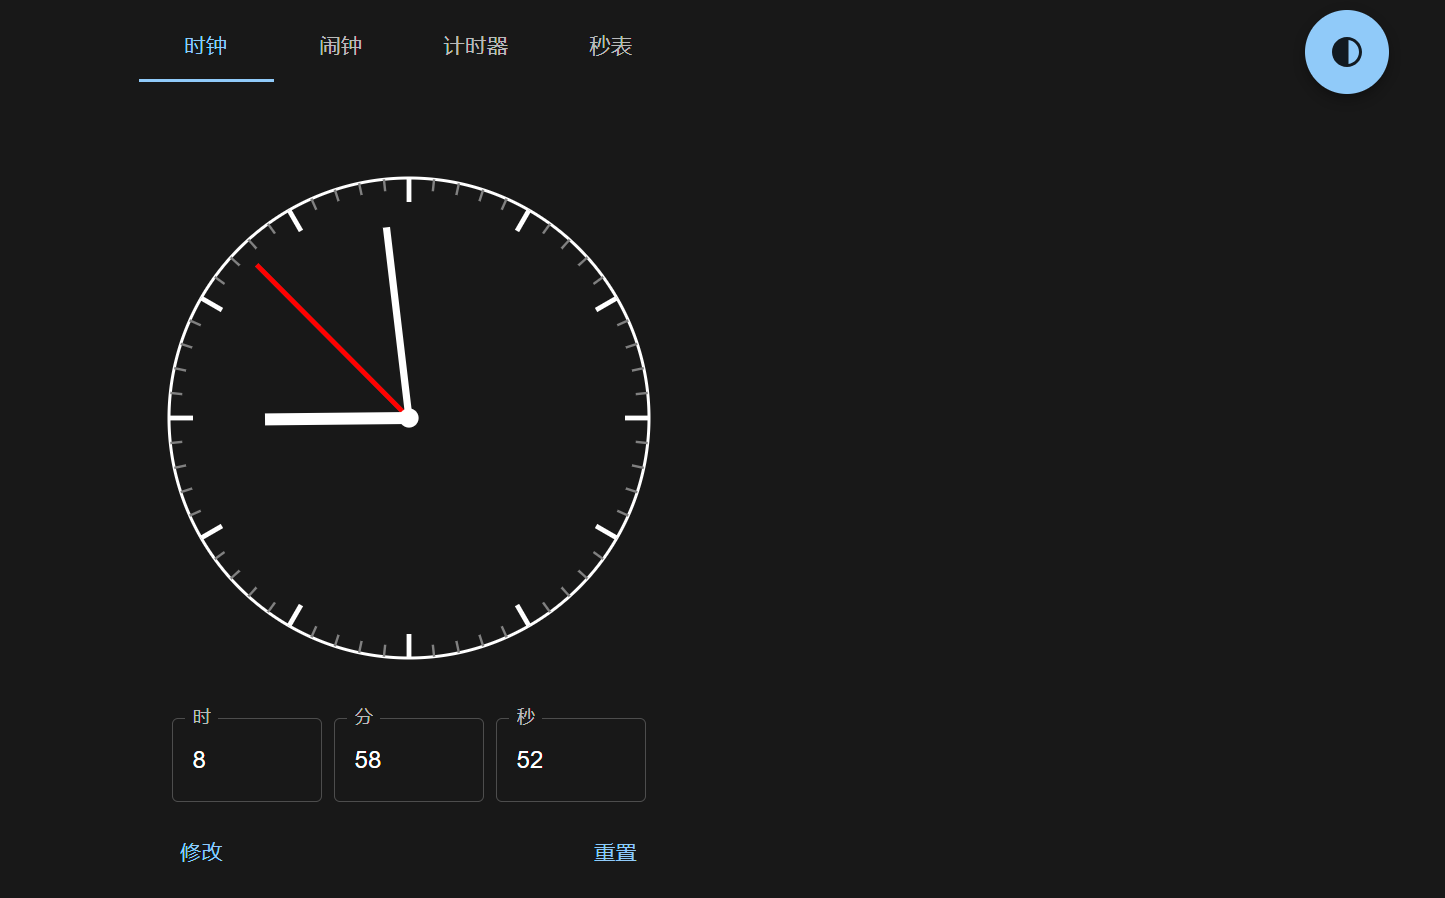
\includegraphics[width=\linewidth]{image/clock_black.png}
        \caption{clock\_black}
    \end{minipage}\hfill
    \begin{minipage}{0.48\textwidth}
        \centering
        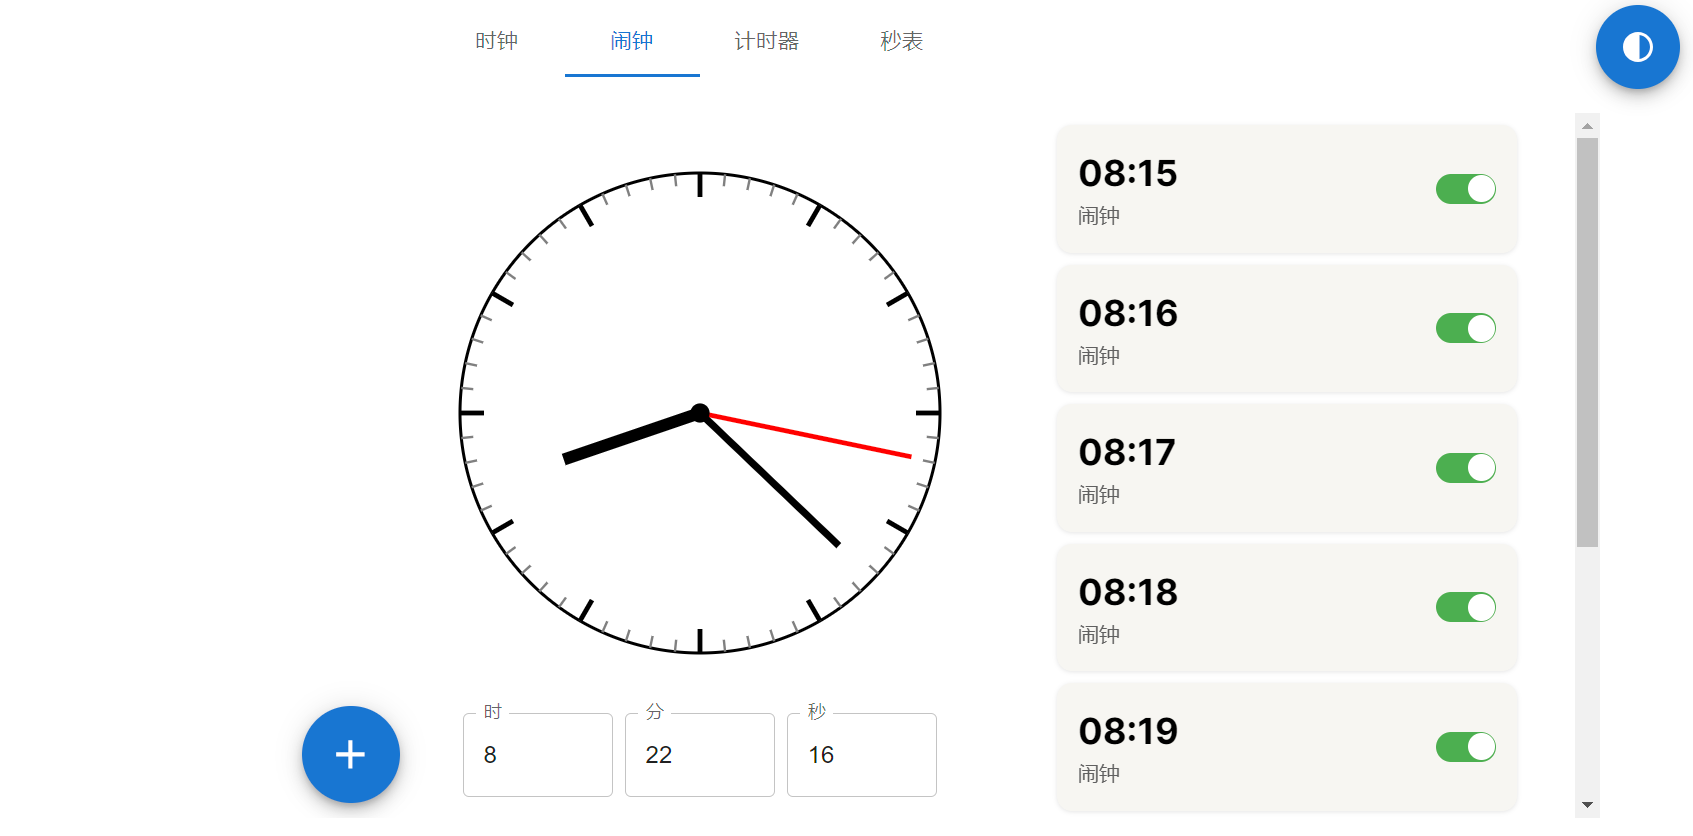
\includegraphics[width=\linewidth]{image/alarm.png}
        \caption{alarm\_light}
    \end{minipage}\hfill
    \begin{minipage}{0.48\textwidth}
        \centering
        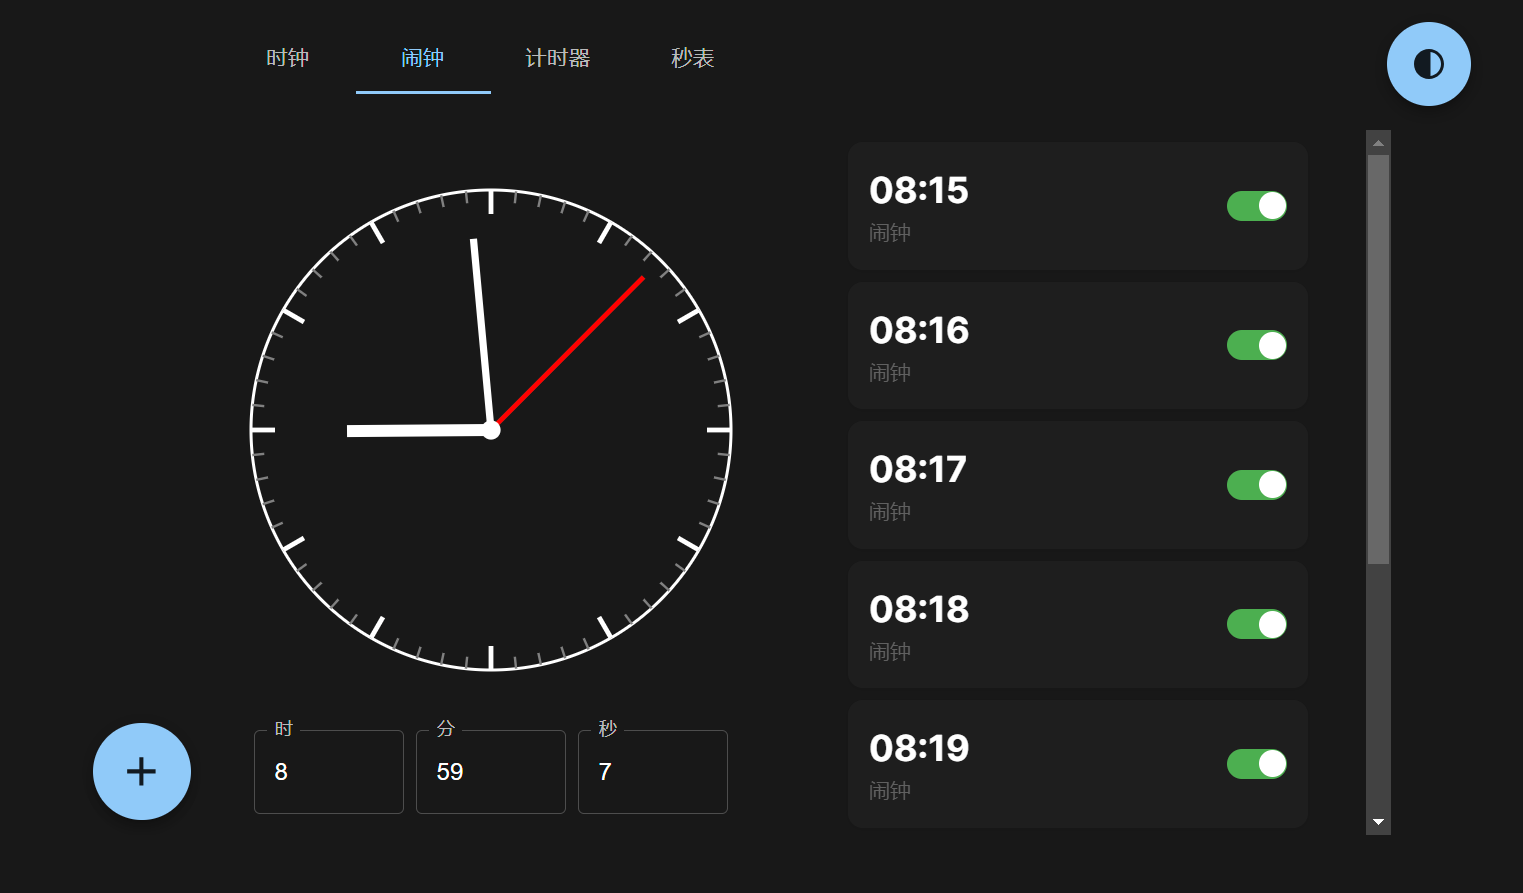
\includegraphics[width=\linewidth]{image/alarm_black.png}
        \caption{alarm\_black}
    \end{minipage}\hfill
    
\end{figure}
\begin{figure}[!h]
    \begin{minipage}{0.48\textwidth}
        \centering
        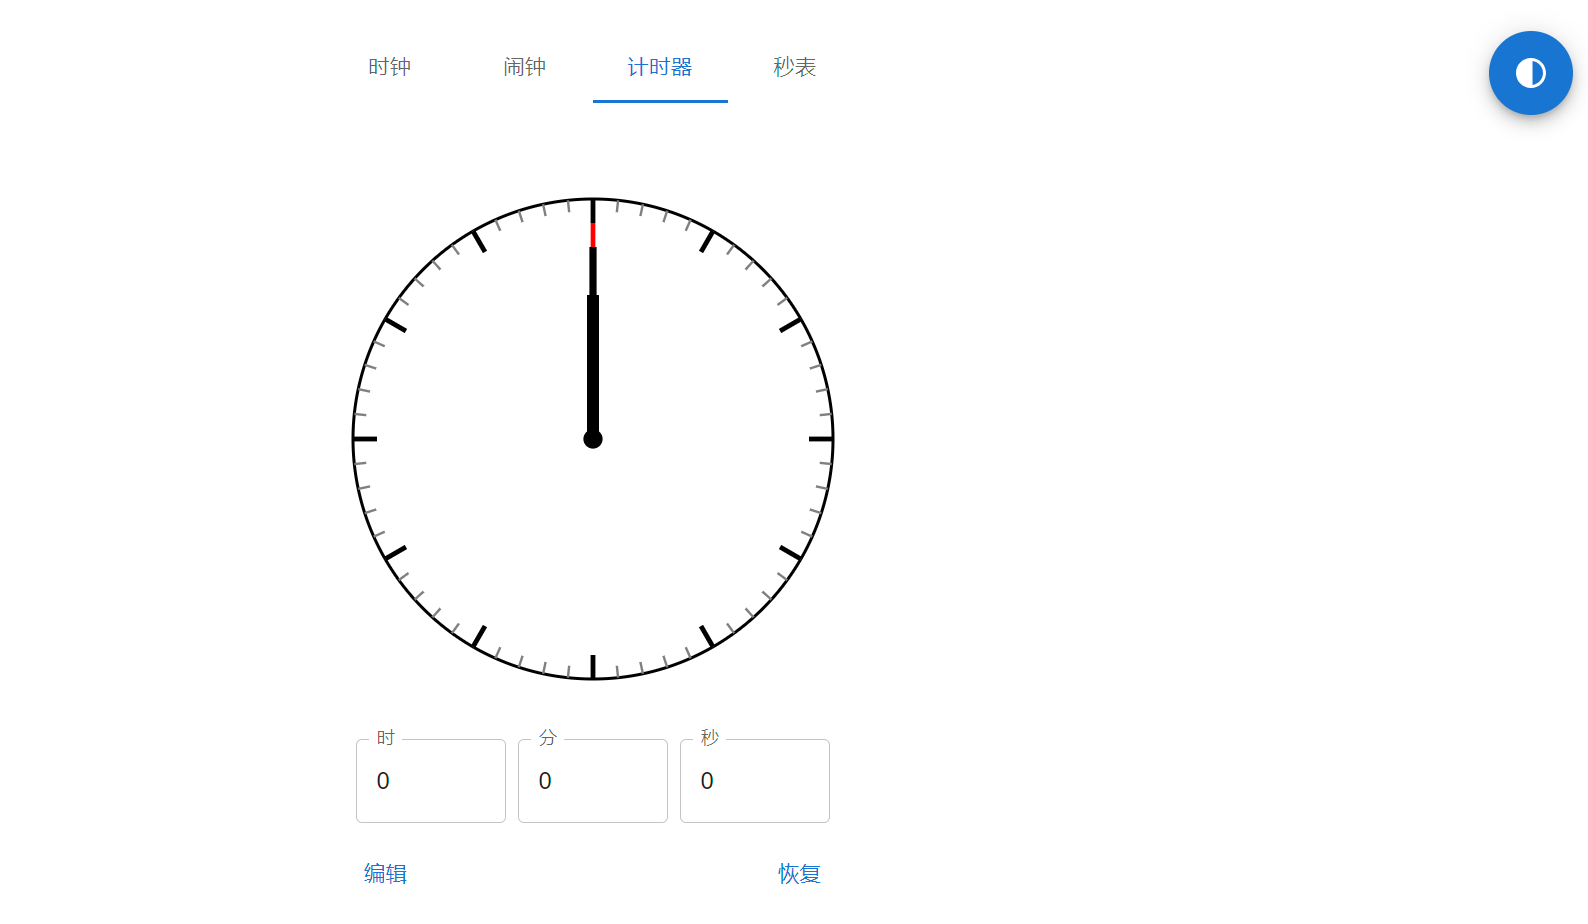
\includegraphics[width=\linewidth]{image/timer.png}
        \caption{timer\_light}
    \end{minipage}\hfill
    \begin{minipage}{0.48\textwidth}
        \centering
        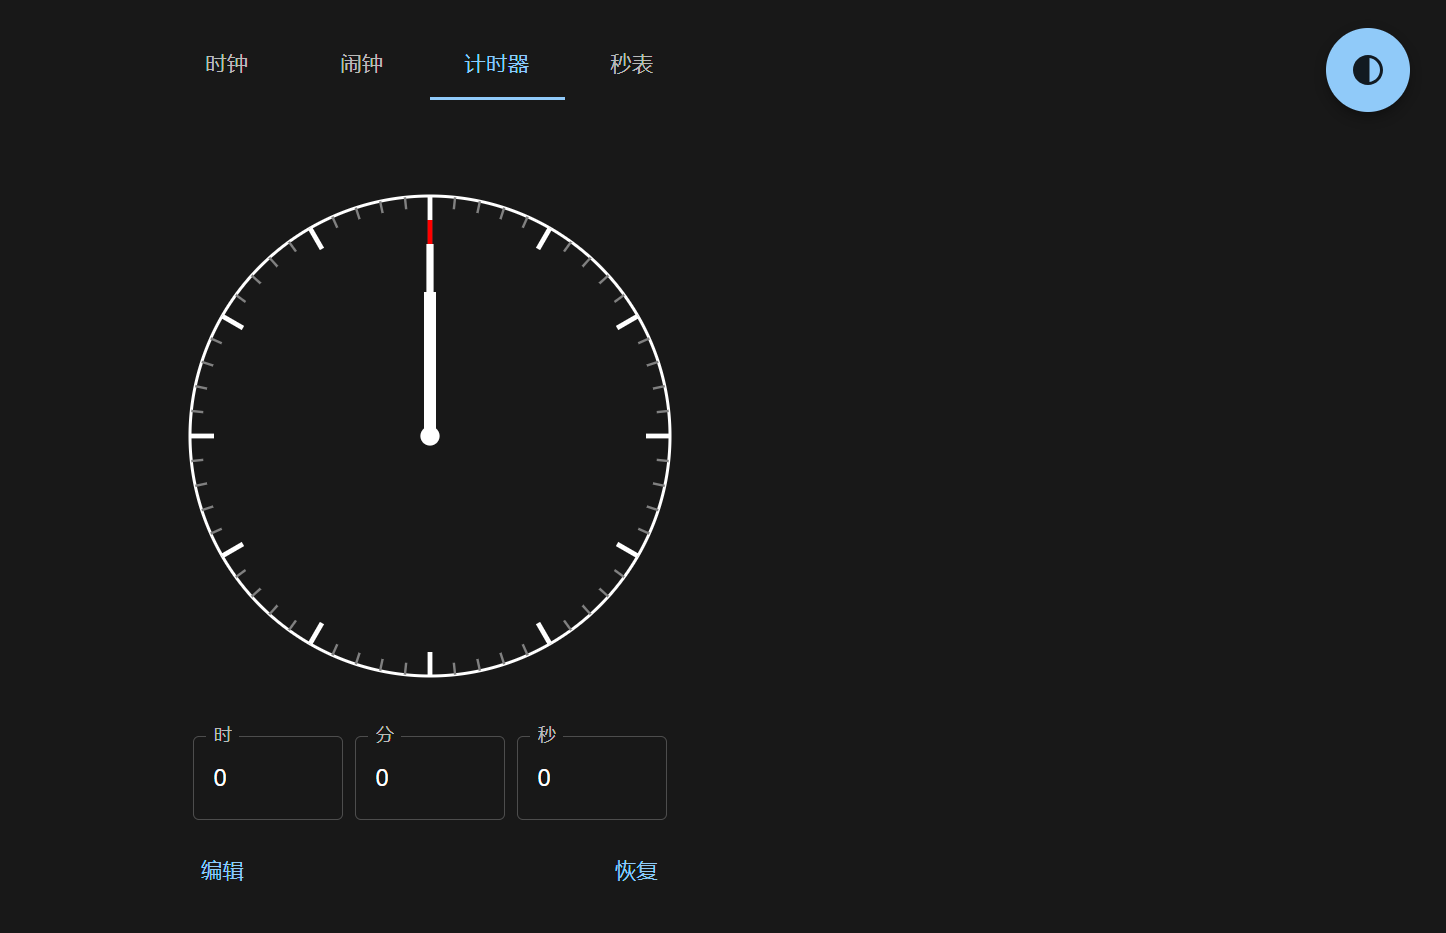
\includegraphics[width=\linewidth]{image/timer_black.png}
        \caption{timer\_black}
    \end{minipage}\hfill
    \begin{minipage}{0.48\textwidth}
        \centering
        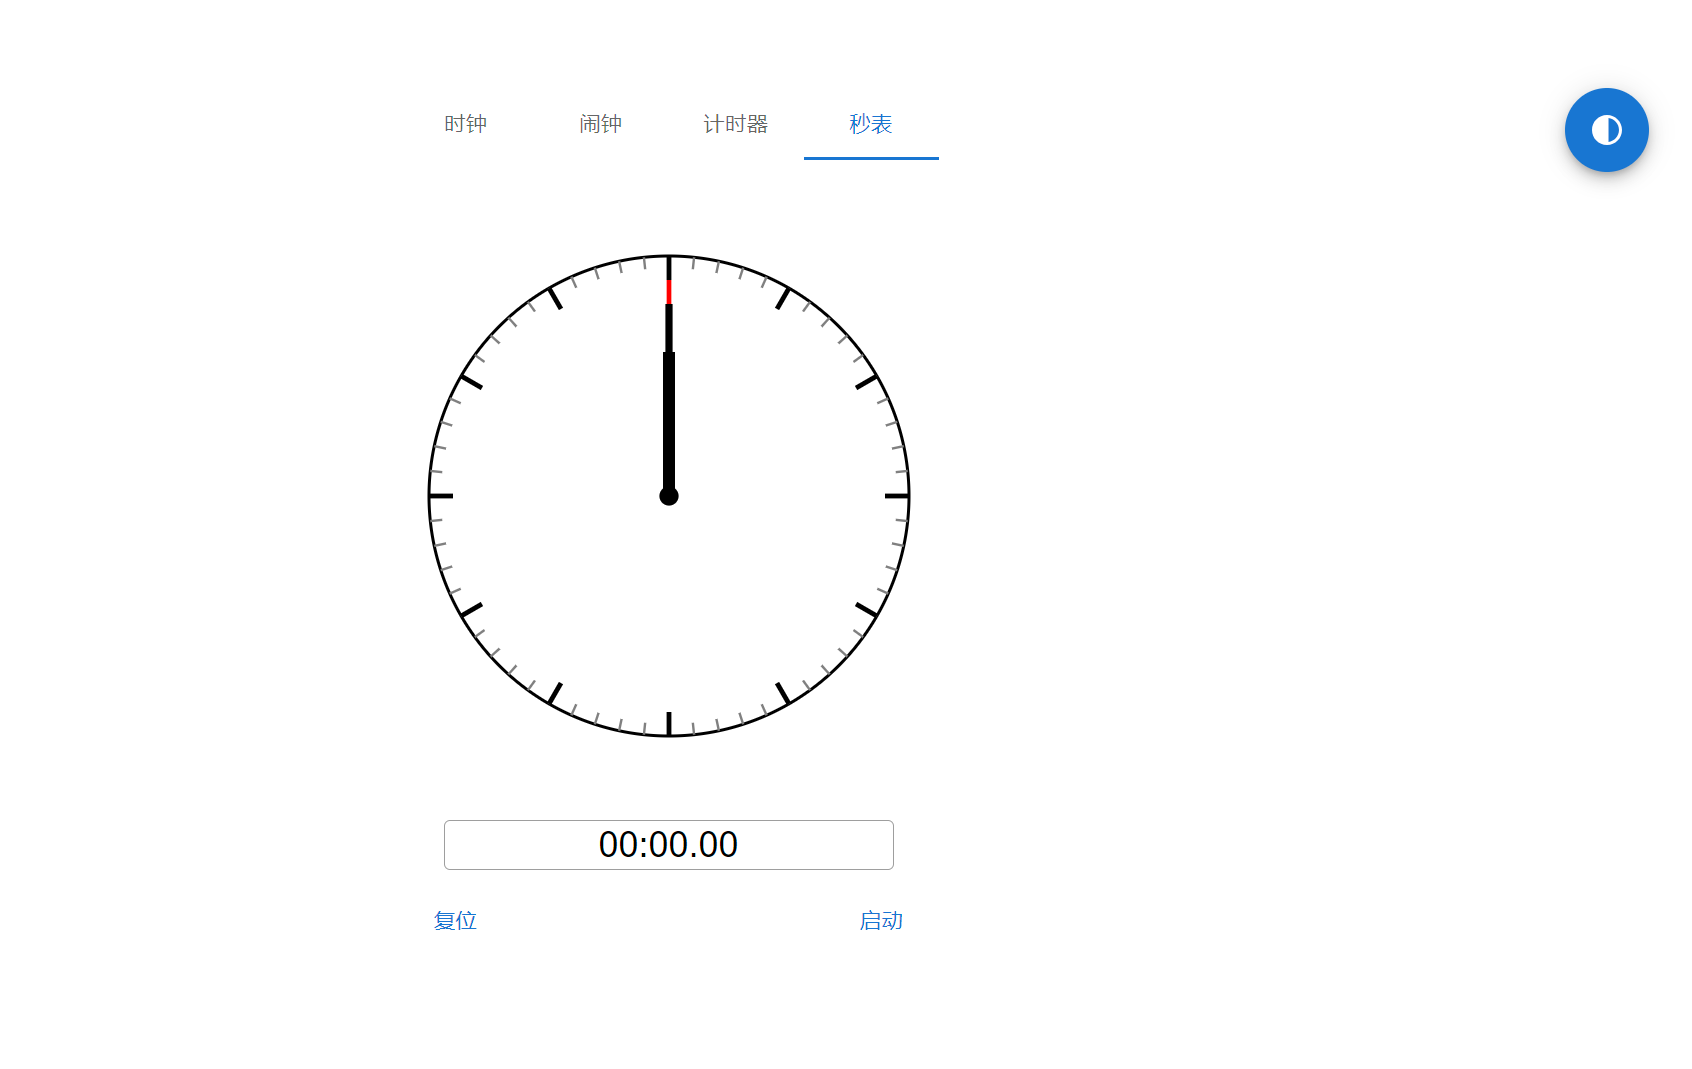
\includegraphics[width=\linewidth]{image/stopwatch.png}
        \caption{stopwatch\_light}
    \end{minipage}
    \begin{minipage}{0.48\textwidth}
        \centering
        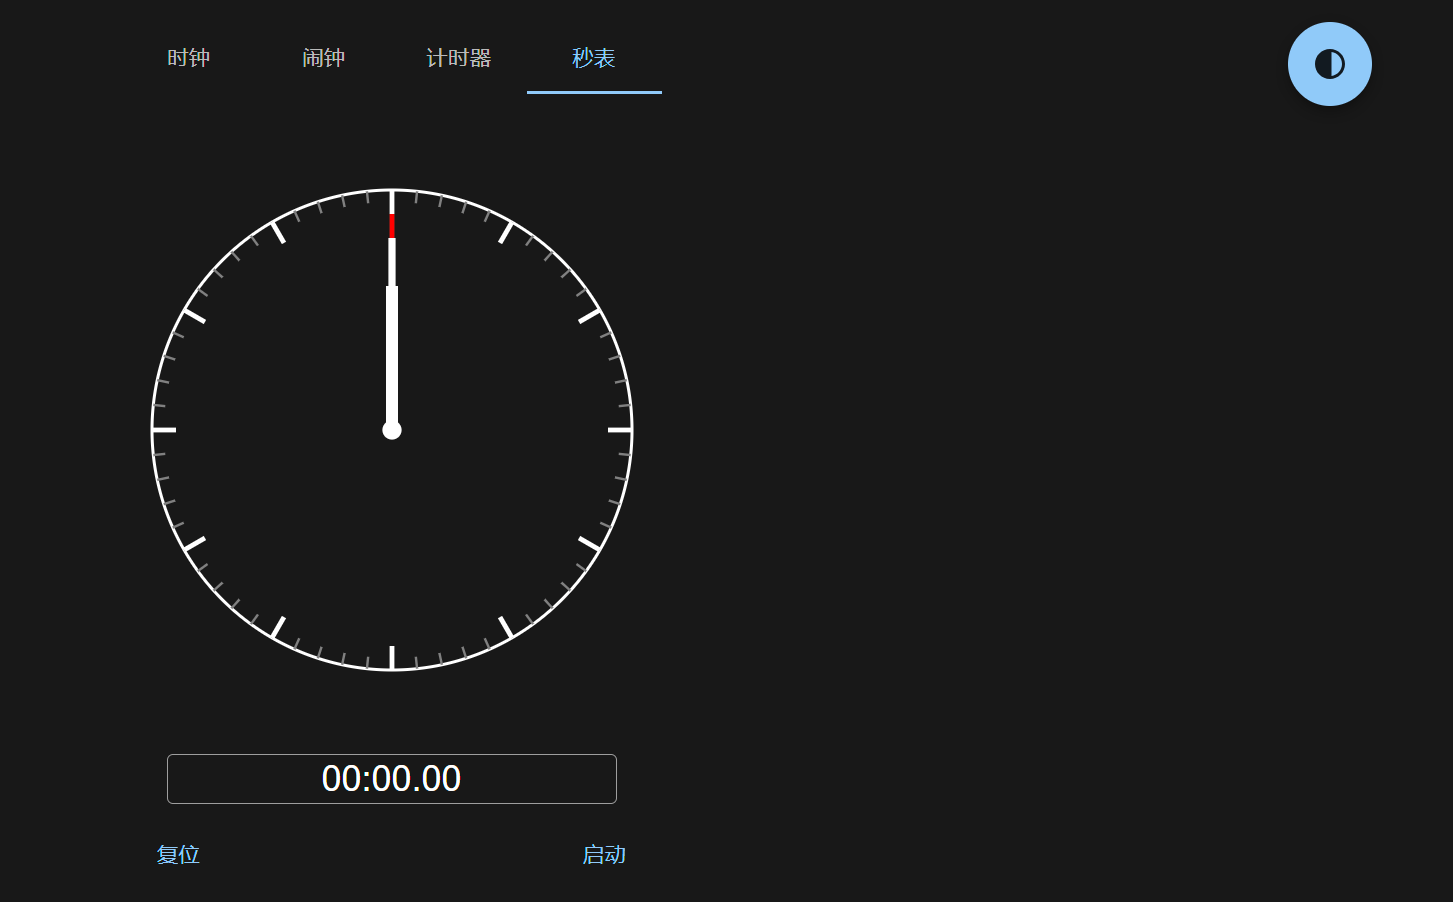
\includegraphics[width=\linewidth]{image/stopwatch_black.png}
        \caption{stopwatch\_black}
    \end{minipage}
\end{figure}
\clearpage
\section{遇到问题及解决方案}
\subsection{时钟}
\subsubsection{问题一及解决方案}

在项目初期,我们采用了错误的实现思路。我们将三个指针写成三个独立的组件,并各自维护更新当前的角度,根据各自当前的角度计算时间。但这样做会带来很多问题,如时针和分针的位置不匹配、指针和数字时间不匹配等。我们将这个错误总结为盲目的解耦。三个指针的位置关系紧密,任何一个指针的位置变化都会影响其他指针。因此,三个指针应该用一种高内聚的方式实现。我们放弃了单独维护三个指针的思路,转换了一种更优雅的思路,即时钟组件单向依赖时间戳,父组件负责更新时间戳,时钟组件通过回调函数响应拖动事件。在采用这种方案之后,我们的开发变得顺利了许多。

\subsubsection{问题二及解决方案}

我们在使用 d3.js 时遇到了类型的问题。d3.js 是一个 JavaScript 的库,因此官方只提供了 JavaScript 文档。我们使用的实际上是 Typescript 版本。官方 d3.js 代码转写为 Typescript 版本时需要手动添加类型。如何在缺乏文档的情况下知道添加哪些类型(甚至在什么位置需要类型)是一个难点。我们对 d3.js 的 ts 接口代码进行了阅读,理解了这些类型的含义,最终解决了问题。
\subsection{闹钟}
\subsubsection{问题三及解决方案}

在最初实现添加和编辑闹钟的提示框时,我们决定新增一个页面localhost:3000/addAlarm,并使用next-js中的拦截路由方式,使其呈现如下效果:当直接访问localhost:3000/addAlarm时,显示完整的addAlarm页面,而点击FAB按钮打开addAlarm时,背景虚化,addAlarm以类似于Modal模态框的形式悬浮在原页面中心。然而,这种处理略显复杂且与其他部分的MUI风格不搭配,因此我们最终采用了弹出MUI风格的Dialog表单实现添加及编辑闹钟。

\subsubsection{问题四及解决方案}

在从LocalStorage中读取alarms数组的过程中,我们发现更新LocalStorage(通过添加或编辑)后的alarms数组不能实时显示在alarmTab中的Alarms组件中。最终,我们通过使用window.addEventListener('alarms-updated', updateAlarms)以及window.dispatchEvent(new Event('alarms-updated'))来监听alarms数组更新事件,一旦检测到该事件,立即调用updateAlarms()函数,更新UI。
\subsection{计时器}
\subsubsection{问题五及解决方案}

在编辑时间时,如果用户输入非数字字符或者留空,可能会引发错误或导致计时器的时间设置不正确。于是在设置时间的输入框中添加适当的验证逻辑。确保用户输入的是有效的数字,并且在输入非数字时提供反馈或者自动纠正为合理的默认值(如0)。

\subsubsection{问题六及解决方案}
 原先使用 Snackbar 组件来显示计时结束的通知,但 Snackbar 主要用于显示简短的信息,而对于需要显示更详细信息(例如超时多长时间)或者需要用户交互的场景,Snackbar 可能不够显眼或不容易提供足够的交互空间。于是替换 Snackbar 为 Dialog 组件。Dialog 提供了更多的空间和灵活性,能够展示更复杂的内容,并且可以包含按钮和其他交互元素,使得用户可以进行更多的操作(如确认消息、查看详情等)。此外,Dialog 在视觉上更加突出,更能够引起用户的注意,确保重要的计时结束通知不会被用户忽视。
\subsection{秒表}

\subsubsection{问题七及解决方案}

最初编写计时逻辑时,采用了计时时间自增的方法,这导致当页面被置于后台时无法正常工作。发现这一问题后,将计时逻辑改为基于实际时间的计算方法。在组件启动时记录开始时间,每次更新时通过当前时间减去开始时间来计算已经过去的时间,从而得到当前计时时间。这种方法避免了页面被置于后台时计时不准确的问题,因为它依赖于系统时间而非前端计时器的持续运行。通过这种方式,即使页面被置于后台或浏览器性能受到影响,计时器仍能准确反映实际经过的时间。

\subsection{明暗模式切换}

\subsubsection{问题八及解决方案}

在最初使用next-themes时,发现黑暗模式下刷新会导致背景颜色加载不正常。经过改进,我们在使用attribute="class"属性,在app/globals.css中的.dark中写入`background-color: black;`,有效解决了黑暗模式下刷新导致背景颜色加载不正常的问题。

\section{参考资料}

\subsection{时钟}
\begin{itemize}
    \item \url{https://d3js.org/}
    \item \url{https://react.dev/}
    \item \url{https://nextjs.org/}
\end{itemize}

\subsection{闹钟}
\begin{itemize}
    \item \url{https://mui.com/material-ui/all-components/}
    \item \url{https://v4.mui.com/components/dialogs/}
\end{itemize}

\subsection{计时器}
\begin{itemize}
    \item \url{https://mui.com/material-ui/react-alert/}
    \item \url{https://juejin.cn/post/6844904006641254407}
\end{itemize}

\subsection{秒表}
\begin{itemize}
    \item \url{https://react.dev/}
    \item \url{https://mui.com/}
\end{itemize}

\subsection{明暗模式切换}
\begin{itemize}
    \item \url{https://github.com/pacocoursey/next-themes}
    \item \url{https://mui.com/material-ui/customization/dark-mode/}
\end{itemize}

\end{document}
